
\section{State Machine}
\begin{figure}[h!]
\label{FIG:GLOBALSTATUSES}
\caption{State diagram that shows possible trasitions between states}
\begin{center}
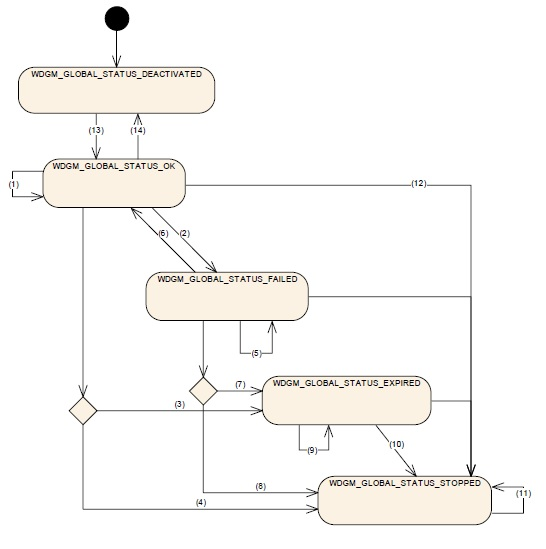
\includegraphics{pictures/globalstatuses.jpg}
\end{center}
\end{figure}



\section{Plots}

\subsection{bsi}
\begin{figure}[h!]
\label{FIG:COMMANDS_BSI}
\caption{bsi configuration}
\begin{center}
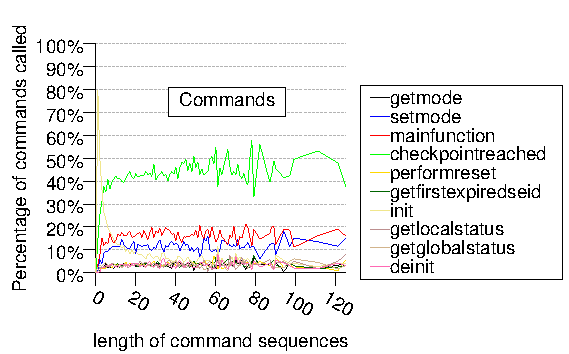
\includegraphics{generated_pictures/history_commands_bsi.pdf}
\end{center}
\end{figure}

\begin{figure}[h!]
\label{FIG:STATUSES_BSI}
\caption{bsi configuration}
\begin{center}
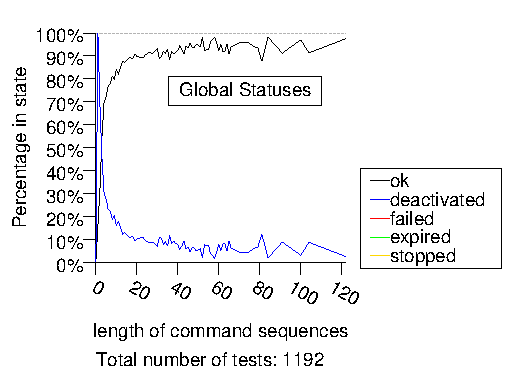
\includegraphics{generated_pictures/history_statuses_bsi.pdf}
\end{center}
\end{figure}

\begin{table}[h!]
\label{TABLE:STATUSES_BSI}

    \begin{tabular}{r|ccccc}
        \hline
        \multicolumn{6}{c}{Number of tests: 2850} \\
        \hline
        \backslashbox{From}{To}
                    & DEACTIVATED & EXPIRED & FAILED & OK & STOPPED \\
        \hline
        DEACTIVATED & \bf{02.23}\% & 00.00\%       & 00.00\%       & \bf{09.12}\% & 00.00\% \\
        EXPIRED     & 00.00\%       & \bf{00.00}\% & 00.00\%       & 00.00\%       & \bf{00.00}\% \\
        FAILED      & 00.00\%       & \bf{00.00}\% & \bf{00.00}\% & \bf{00.00}\% & \bf{00.00}\% \\
        OK          & \bf{03.24}\% & \bf{00.00}\% & \bf{00.00}\% & \bf{85.41}\% & \bf{00.00}\% \\
        STOPPED     & 00.00\%       & 00.00\%       & 00.00\%       & 00.00\%       & \bf{00.00}\%
      \end{tabular}
    

\caption{bsi configuration}
\end{table}

\subsection{freescale}

\begin{figure}[h!]
\label{FIG:COMMANDS_FREESCALE}
\caption{freescale configuration}
\begin{center}
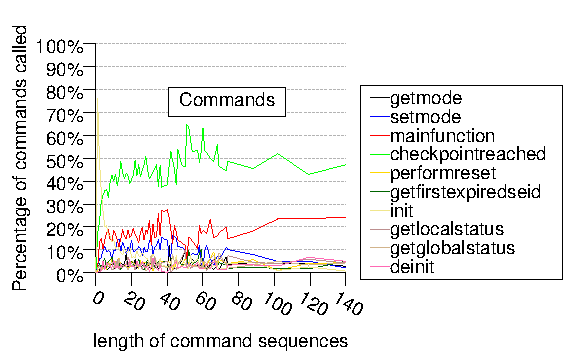
\includegraphics{generated_pictures/history_commands_freescale.pdf}
\end{center}
\end{figure}

\begin{figure}[h!]
\label{FIG:STATUSES_FREESCALE}
\caption{freescale configuration}
\begin{center}
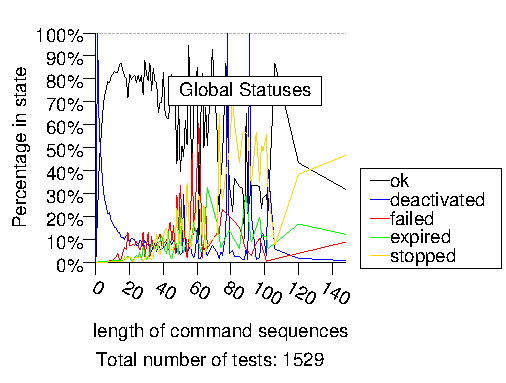
\includegraphics{generated_pictures/history_statuses_freescale.pdf}
\end{center}
\end{figure}

\begin{table}[!h]
\label{TABLE:STATUSES_FREESCALE}

    \begin{tabular}{r|ccccc}
        \hline
        \multicolumn{6}{c}{Number of tests: 1023} \\
        \hline
        \backslashbox{From}{To}
                    & DEACTIVATED & EXPIRED & FAILED & OK & STOPPED \\
        \hline
        DEACTIVATED & \bf{02.43}\% & 00.00\%       & 00.00\%       & \bf{08.32}\% & 00.00\% \\
        EXPIRED     & 00.00\%       & \bf{03.36}\% & 00.00\%       & 00.00\%       & \bf{00.11}\% \\
        FAILED      & 00.00\%       & \bf{00.17}\% & \bf{07.77}\% & \bf{00.12}\% & \bf{00.11}\% \\
        OK          & \bf{02.56}\% & \bf{00.18}\% & \bf{00.87}\% & \bf{69.53}\% & \bf{00.12}\% \\
        STOPPED     & 00.00\%       & 00.00\%       & 00.00\%       & 00.00\%       & \bf{04.34}\%
      \end{tabular}
    

\caption{freescale configuration}
\end{table}

\subsection{example}

\begin{figure}[h!]
\label{FIG:COMMANDS_EXAMPLE}
\caption{example configuration}
\begin{center}
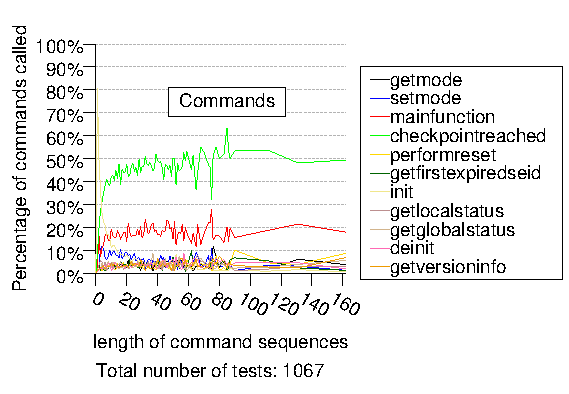
\includegraphics{generated_pictures/history_commands_example.pdf}
\end{center}
\end{figure}

\begin{figure}[h!]
\label{FIG:STATUSES_EXAMPLE}
\caption{example configuration}
\begin{center}
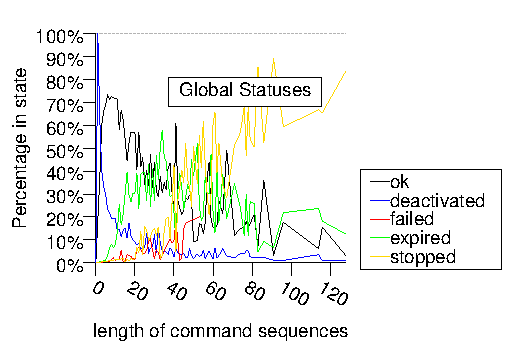
\includegraphics{generated_pictures/history_statuses_example.pdf}
\end{center}
\end{figure}

\begin{table}[!h]
\label{TABLE:STATUSES_EXAMPLE}

    \begin{tabular}{r|ccccc}
        \hline
        \multicolumn{6}{c}{Number of tests: 3877} \\
        \hline
        \backslashbox{From}{To}
                    & DEACTIVATED & EXPIRED & FAILED & OK & STOPPED \\
        \hline
        DEACTIVATED & \bf{02.59}\% & 00.00\%       & 00.00\%       & \bf{07.81}\% & 00.00\% \\
        EXPIRED     & 00.00\%       & \bf{24.77}\% & 00.00\%       & 00.00\%       & \bf{00.81}\% \\
        FAILED      & 00.00\%       & \bf{00.12}\% & \bf{02.87}\% & \bf{00.00}\% & \bf{00.04}\% \\
        OK          & \bf{01.68}\% & \bf{02.50}\% & \bf{00.39}\% & \bf{40.22}\% & \bf{00.14}\% \\
        STOPPED     & 00.00\%       & 00.00\%       & 00.00\%       & 00.00\%       & \bf{16.07}\%
      \end{tabular}
    

\caption{example configuration}
\end{table}

\section{Handle bugs in the C code}
\label{sec:handlebugs}

\section{Statistics}
